% XCircuit output "priebehy_1.tex" for LaTeX input from priebehy_1.ps
\def\putbox#1#2#3#4{\makebox[0in][l]{\makebox[#1][l]{}\raisebox{\baselineskip}[0in][0in]{\raisebox{#2}[0in][0in]{\scalebox{#3}{#4}}}}}
\def\rightbox#1{\makebox[0in][r]{#1}}
\def\centbox#1{\makebox[0in]{#1}}
\def\topbox#1{\raisebox{-0.60\baselineskip}[0in][0in]{#1}}
\def\midbox#1{\raisebox{-0.20\baselineskip}[0in][0in]{#1}}
   \scalebox{0.8}{
   \normalsize
   \parbox{4.44792in}{
   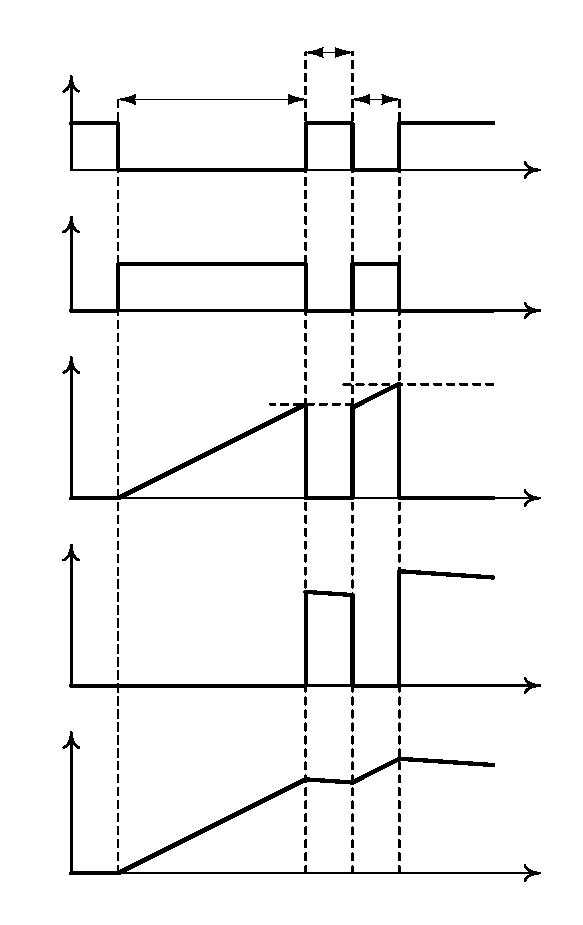
\includegraphics[scale=1.25]{priebehy_1}\\
   % translate x=314 y=1408 scale 0.30
   \putbox{4.17in}{4.78in}{1.20}{\llgt}%
   \putbox{0.06in}{5.57in}{1.20}{\llgvL}%
   \putbox{0.06in}{4.39in}{1.20}{\llgic}%
   \putbox{0.06in}{2.83in}{1.20}{\llgiD}%
   \putbox{0.06in}{1.27in}{1.20}{\llgiL}%
   \putbox{4.17in}{3.22in}{1.20}{\llgt}%
   \putbox{4.17in}{1.66in}{1.20}{\llgt}%
   \putbox{4.17in}{0.10in}{1.20}{\llgt}%
   \putbox{1.43in}{6.84in}{1.20}{\rotatebox{-360}{\llgTonj}}%
   \putbox{2.80in}{6.84in}{1.20}{\llgTond}%
   \putbox{0.06in}{6.74in}{1.20}{\llgvce}%
   \putbox{4.17in}{5.96in}{1.20}{\llgt}%
   \putbox{2.41in}{7.24in}{1.20}{\llgToffj}%
   \putbox{2.31in}{0.10in}{1.20}{\llgtj}%
   \putbox{2.71in}{0.10in}{1.20}{\llgtd}%
   \putbox{2.07in}{4.30in}{1.20}{\llgIc}%
   \putbox{3.27in}{4.47in}{1.20}{\llUmerBmax}%
   } % close 'parbox'
   } % close 'scalebox'
   \vspace{-\baselineskip} % this is not necessary, but looks better
